\iffalse
\let\negmedspace\undefined
\let\negthickspace\undefined
\documentclass[journal,12pt,twocolumn]{IEEEtran}
\usepackage{cite}
\usepackage{amsmath,amssymb,amsfonts,amsthm}
\usepackage{algorithmic}
\usepackage{graphicx}
\usepackage{textcomp}
\usepackage{xcolor}
\usepackage{txfonts}
\usepackage{listings}
\usepackage{enumitem}
\usepackage{mathtools}
\usepackage{gensymb}
\usepackage{comment}
\usepackage[breaklinks=true]{hyperref}
\usepackage{tkz-euclide} 
\usepackage{listings}
\usepackage{gvv}                                        
\def\inputGnumericTable{}                                 
\usepackage[latin1]{inputenc}                                
\usepackage{color}                                            
\usepackage{array}                                            
\usepackage{longtable}                                       
\usepackage{calc}                                             
\usepackage{multirow}                                         
\usepackage{hhline}                                           
\usepackage{ifthen}                                           
\usepackage{lscape}

\newtheorem{theorem}{Theorem}[section]
\newtheorem{problem}{Problem}
\newtheorem{proposition}{Proposition}[section]
\newtheorem{lemma}{Lemma}[section]
\newtheorem{corollary}[theorem]{Corollary}
\newtheorem{example}{Example}[section]
\newtheorem{definition}[problem]{Definition}
\newcommand{\BEQA}{\begin{eqnarray}}
\newcommand{\EEQA}{\end{eqnarray}}
\newcommand{\define}{\stackrel{\triangle}{=}}
\theoremstyle{remark}
\newtheorem{rem}{Remark}
\begin{document}
\parindent 0px
\bibliographystyle{IEEEtran}
\title{GATE: ES - 36.2022}
\author{EE22BTECH11219 - Rada Sai Sujan$^{}$% <-this % stops a space
}
\maketitle
\newpage
\bigskip
\section*{Question}
Given, $y=f\brak{x}$; $\frac{d^2y}{dx2}+4y=0; y\brak{0}=0; \frac{dy}{dx}\brak{0}=1$. The problem is a/an \\
\begin{enumerate}[label=(\alph*)]
    \item initial value problem having soluition $y=x$
    \item boundary value problem having soluition $y=x$
    \item initial value problem having soluition $y=\frac{1}{2}\sin 2x$
    \item boundary value problem having soluition {$y=\frac{1}{2}\sin 2x$}
\end{enumerate} \hfill(GATE 2022 ES)    \\
\solution
\fi

The above equation can be written as,
\begin{align}
    y^{\prime\prime}\brak{t}+4y\brak{t}=0
\end{align}
Using the Laplace transformation pairs,
\begin{align}
    y^{\prime\prime}\brak{t} &\overset{\mathcal{L}}{ \longleftrightarrow} s^2Y\brak{s}-sy\brak{0}-y^{\prime}\brak{0}    \\
    y\brak{t} &\overset{\mathcal{L}}{ \longleftrightarrow} Y\brak{s}    \\
    \sin at &\overset{\mathcal{L}}{ \longleftrightarrow} \frac{a}{a^2+s^2}  \label{equation:gate.es.2022.4}
\end{align}
Applying Laplace transform for the equation we get,
\begin{align}
    s^2Y\brak{s}-1+4Y\brak{s} &= 0  \\
    \implies Y\brak{s} &= \frac{1}{4+s^2}
\end{align}
Now, applying inverse laplace transform we get,
\begin{align}
    y\brak{t} &= \frac{1}{2}\sin 2t \quad \text{(from \eqref{equation:gate.es.2022.4})}
\end{align}
Since, the conditions at the same point\brak{0} are mentioned, it is an initial valued problem having solution $y=\frac{1}{2}\sin 2x$.
\begin{figure}
    \centering
    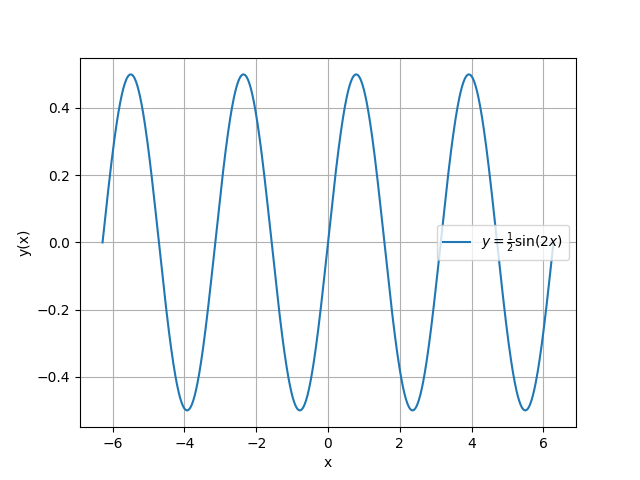
\includegraphics[width=\columnwidth]{2022/ES/36/figs/a.png}
    \caption{$y\brak{x}$ $vs$ $x$ graph}
    \label{figure:gate.2022.es.36Q.1}
\end{figure}
